\documentclass[tikz,border=4pt]{standalone}
\usepackage[T1]{fontenc}
\usepackage{helvet,amsmath,amssymb}
\renewcommand{\familydefault}{\sfdefault}
\usetikzlibrary{arrows.meta,positioning,fit,calc,shapes.geometric,backgrounds}
\definecolor{navy}{HTML}{193A56}
\definecolor{teal}{HTML}{167D8D}
\definecolor{amber}{HTML}{B87420}
\definecolor{pale}{HTML}{EDF3F6}
\definecolor{mint}{HTML}{EAF5F2}
\definecolor{warm}{HTML}{FFF3E3}
\definecolor{gray}{HTML}{586772}
\tikzset{box/.style={draw=navy!60,rounded corners=2pt,fill=pale,align=center,inner sep=6pt,font=\sffamily\fontsize{8}{9}\selectfont},unit/.style={box,draw=teal,fill=mint},gate/.style={box,draw=amber,fill=warm},arr/.style={-{Latex[length=2.2mm]},thick,draw=navy},note/.style={font=\sffamily\footnotesize,text=gray,align=left},label/.style={font=\sffamily\bfseries\small,text=navy}}
\begin{document}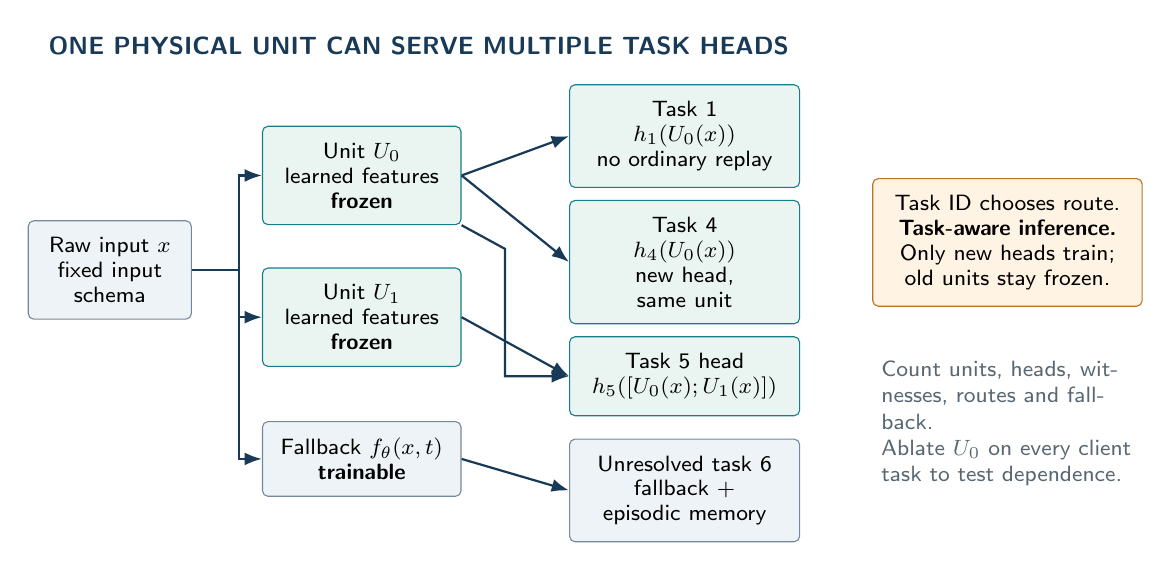
\begin{tikzpicture}[x=1cm,y=1cm]

\node[label,anchor=west] at (0,5.25) {ONE PHYSICAL UNIT CAN SERVE MULTIPLE TASK HEADS};
\node[box,text width=1.65cm] (x) at (.9,2.4) {Raw input $x$\\fixed input schema};
\node[unit,text width=2.1cm,minimum height=1cm] (u0) at (4.1,3.6) {Unit $U_0$\\learned features\\\textbf{frozen}};
\node[unit,text width=2.1cm,minimum height=1cm] (u1) at (4.1,1.8) {Unit $U_1$\\learned features\\\textbf{frozen}};
\node[box,text width=2.1cm] (fallback) at (4.1,0) {Fallback $f_\theta(x,t)$\\\textbf{trainable}};
\node[unit,text width=2.5cm] (h1) at (8.2,4.1) {Task 1\\$h_1(U_0(x))$\\no ordinary replay};
\node[unit,text width=2.5cm] (h4) at (8.2,2.5) {Task 4\\$h_4(U_0(x))$\\new head, same unit};
\node[unit,text width=2.5cm] (h5) at (8.2,1.05) {Task 5 head\\$h_5([U_0(x);U_1(x)])$};
\node[box,text width=2.5cm] (h6) at (8.2,-.4) {Unresolved task 6\\fallback + episodic memory};
\draw[arr] (x.east)--++(.6,0)|-(u0.west);\draw[arr] (x.east)--++(.6,0)|-(u1.west);\draw[arr] (x.east)--++(.6,0)|-(fallback.west);
\draw[arr] (u0.east)--(h1.west);\draw[arr] (u0.east)--(h4.west);
\draw[arr] (u0.south east)--++(.55,-.3)|-(h5.west);\draw[arr] (u1.east)--(h5.west);
\draw[arr] (fallback.east)--(h6.west);
\node[gate,text width=3.0cm] at (12.3,2.75) {Task ID chooses route.\\\textbf{Task-aware inference.}\\Only new heads train;\\old units stay frozen.};
\node[note,text width=3.2cm] at (12.3,.45) {Count units, heads, witnesses, routes and fallback.\par Ablate $U_0$ on every client task to test dependence.};
\end{tikzpicture}\end{document}